\documentclass[11pt]{article}

\usepackage[margin=1in]{geometry}
\usepackage{amsmath,amssymb,bm,booktabs,enumitem,graphicx,hyperref,microtype,natbib}
\usepackage{tikz}
\usepackage[T1]{fontenc}
\usepackage{lmodern}
\usetikzlibrary{arrows.meta,positioning,shapes.geometric}
\setlist[itemize]{leftmargin=2em}
\setlist[enumerate]{leftmargin=2em}
\setlength{\parskip}{0.45em}
\setlength{\parindent}{0pt}
\hypersetup{colorlinks=true, linkcolor=blue, citecolor=blue, urlcolor=blue}

\newcommand{\by}{\bm{y}}
\newcommand{\bbeta}{\bm{\beta}}
\newcommand{\bw}{\bm{\omega}}
\newcommand{\beps}{\bm{\epsilon}}
\newcommand{\btheta}{\bm{\theta}}
\newcommand{\bzero}{\bm{0}}
\newcommand{\bI}{\bm{I}}
\newcommand{\bC}{\bm{C}}
\newcommand{\bD}{\bm{D}}
\newcommand{\bH}{\bm{H}}
\newcommand{\bV}{\bm{V}}
\newcommand{\bQ}{\bm{Q}}
\newcommand{\bX}{\bm{X}}
\newcommand{\bZ}{\bm{Z}}
\newcommand{\bz}{\bm{z}}
\newcommand{\bOmega}{\bm{\Omega}}
\newcommand{\trans}{^\top}

\title{\texttt{cosTapered}: Model and Software Details}
\author{Andrew O. Finley}
\date{Updated \today}

% Cover-page logo size and spacing below the image.
\newcommand{\coverlogowidth}{0.42\textwidth}
\newcommand{\coverlogogap}{0.25in}

\begin{document}
\pagenumbering{gobble}
\begin{titlepage}
  \centering
  \vspace*{0.65in}
  {\Huge\bfseries \texttt{cosTapered}\par}
  \vspace{0.35in}
  {\LARGE Model and Software Details\par}
  \vspace{0.55in}
  {\large Andrew O. Finley\par}
  \vspace{0.25in}
  {\large Updated \today\par}
  \vfill
  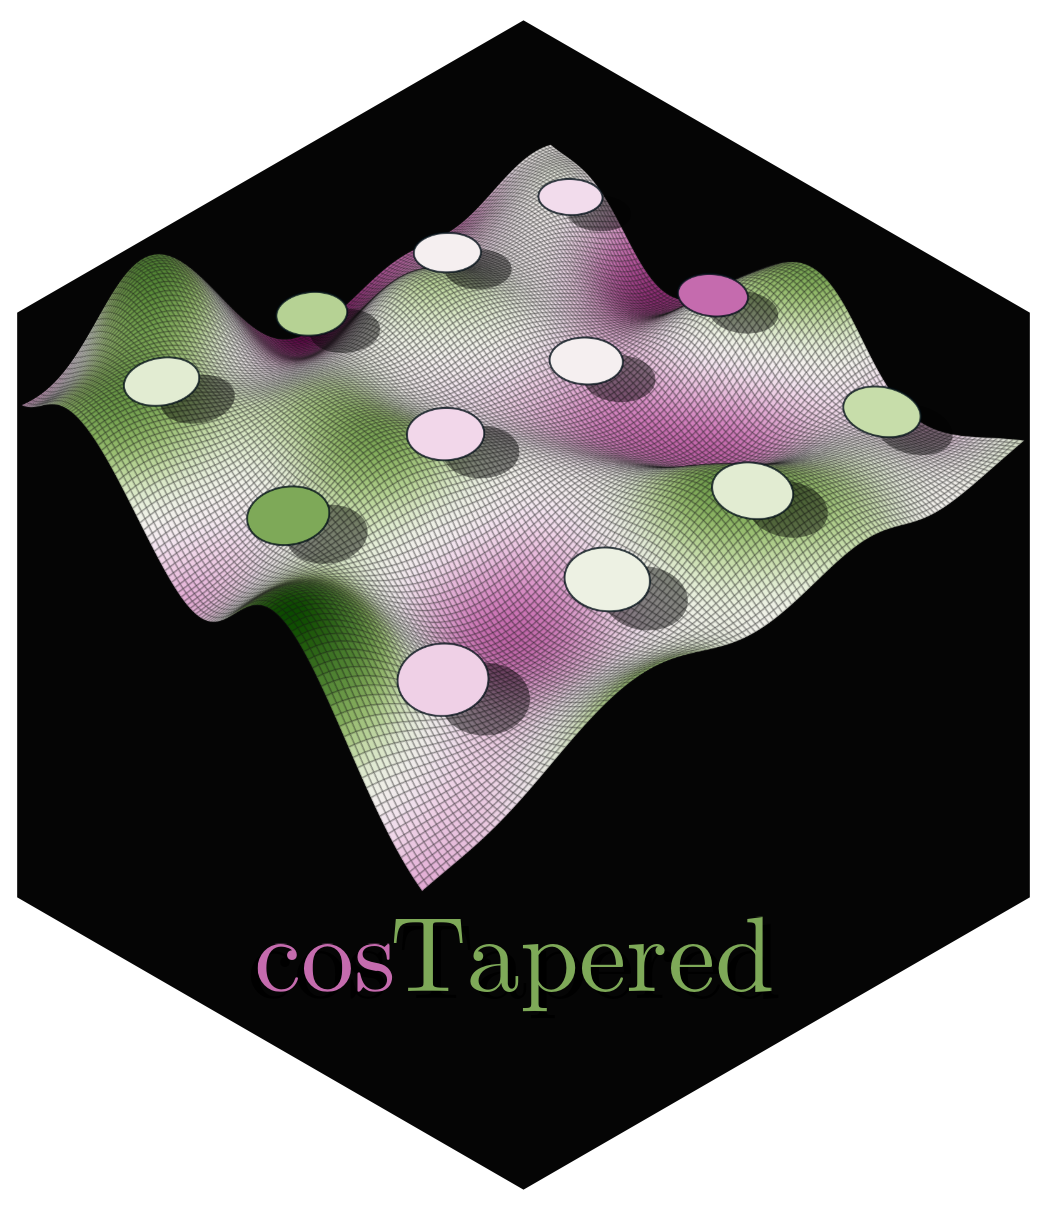
\includegraphics[width=\coverlogowidth]{figures/logo.png}\par
  \vspace{\coverlogogap}
  {\large Bayesian change-of-support modeling with tapered exponential covariance\par}
  \vfill
\end{titlepage}

\clearpage
\pagenumbering{roman}
\tableofcontents
\clearpage
\pagenumbering{arabic}

\section{Purpose}

This document records the model and computing details behind the current
\texttt{cosTapered} implementation. It is intended as a compact mathematical
reference for package users and developers. The introductory and model
vignettes remain the best place to learn the user workflow; this document
collects notation, model equations, posterior calculations, and software
conventions in one place.

The package is intentionally narrower than the broader change-of-support
framework that motivated it. The Gaussian response model follows the tapered
exponential residual spatial process used in the forest damage application of
\citet{ZhangEtAl2024}. The current development version also includes
binomial logit and fixed-size negative-binomial response models fit with
Polya-Gamma data augmentation \citep{PolsonScottWindle2013,Windle2013}. The
support-weight layer is shared by these response models; what changes is the
observation model and the associated sampling step.

\section{Spatial supports and design matrix}

Let \(A_i\), \(i=1,\ldots,n_A\), denote fine raster cells. Let \(s_i\) denote
the centroid of cell \(A_i\). Let \(B_l\), \(l=1,\ldots,n_B\), denote observed
supports, such as field plots, and let \(U_k\), \(k=1,\ldots,n_U\), denote
prediction supports, such as stands or holdout polygons.

The fine-support covariate vector is \(\bm{x}(A_i)\in\mathbb{R}^p\). The
fine-support design matrix is
\begin{equation}
  \bX =
  \begin{bmatrix}
    \bm{x}(A_1)\trans\\
    \vdots\\
    \bm{x}(A_{n_A})\trans
  \end{bmatrix}.
\end{equation}
The package uses the columns supplied in \texttt{X\_rast}. It does not add an
intercept, transform covariates, or scale raster layers automatically. If an
intercept is wanted, the user supplies an intercept raster layer.

Observed-support weights are
\begin{equation}
  h_{li} = \frac{|B_l\cap A_i|}{|B_l|},
\end{equation}
and define the sparse aggregation matrix \(\bH_{BA}\). Prediction-support
weights are
\begin{equation}
  g_{ki} = \frac{|U_k\cap A_i|}{|U_k|},
\end{equation}
and define the conceptual aggregation matrix \(\bH_{UA}\). The package stores
\(\bH_{BA}\) as a sparse matrix and stores prediction weights block by block.

\section{Fine-support Gaussian model}

The current Gaussian response model is written at the finite raster-cell
support as
\begin{equation}
  y(A_i) = \eta(A_i) + \epsilon(A_i),
  \qquad
  \eta(A_i) = \bm{x}(A_i)\trans\bbeta + \omega(A_i).
\end{equation}
In vector form,
\begin{equation}
  \by_A = \bm{\eta}_A+\beps_A,
  \qquad
  \bm{\eta}_A = \bX\bbeta+\bw_A,
\end{equation}
with
\begin{equation}
  \beps_A\mid\tau^2\sim N(\bzero,\tau^2\bI_{n_A}).
\end{equation}
The independent noise term is a finite-cell nugget. It is not modeled as a
continuous point-level white-noise process. This convention determines how
nugget variance changes under support averaging.

The residual spatial process is
\begin{equation}
  \bw_A\mid\sigma^2,\phi,\gamma
  \sim N\{\bzero,\sigma^2\bC_A^{tap}(\phi,\gamma)\}.
\end{equation}
For cells \(i\) and \(j\),
\begin{equation}
  [\bC_A^{tap}(\phi,\gamma)]_{ij}
  =
  \exp\{-\phi d(s_i,s_j)\}T_\gamma\{d(s_i,s_j)\},
\end{equation}
where \(d(\cdot,\cdot)\) is Euclidean distance in the projected coordinate
system. The current package supports the Wendland taper and the spherical
taper. For \(r=d/\gamma\), the Wendland taper used by
\texttt{taper\_code = 1L} is
\begin{equation}
  T_\gamma(d) =
  (1-r)^4(1+4r)\bm{1}(0\leq r < 1),
\end{equation}
and the spherical taper used by \texttt{taper\_code = 2L} is
\begin{equation}
  T_\gamma(d) =
  \left(1-\frac{3}{2}r+\frac{1}{2}r^3\right)\bm{1}(0\leq r < 1).
\end{equation}
Both tapers are zero for distances greater than or equal to \(\gamma\). The
exponential effective range reported by the package is the
distance at which the exponential component alone drops to 0.05:
\begin{equation}
  r_{0.05} = -\log(0.05)/\phi \approx 3/\phi.
\end{equation}
This effective range is not the taper distance \(\gamma\). The taper distance
is a compact-support cutoff chosen by the user.

\section{Observed-support model}

Observed responses are support averages of the fine-support response:
\begin{equation}
  y(B_l) \approx \sum_i h_{li}y(A_i).
\end{equation}
Stacking observed responses gives
\begin{equation}
  \by_B =
  \bH_{BA}\bX\bbeta +
  \bH_{BA}\bw_A +
  \bH_{BA}\beps_A.
\end{equation}
Define
\begin{equation}
  \bX_B=\bH_{BA}\bX,\qquad
  \bw_B=\bH_{BA}\bw_A,\qquad
  \bD_h=\bH_{BA}\bH_{BA}\trans .
\end{equation}
Then
\begin{equation}
  \by_B\mid\bbeta,\bw_B,\tau^2
  \sim
  N(\bX_B\bbeta+\bw_B,\tau^2\bD_h),
\end{equation}
and
\begin{equation}
  \bw_B\mid\sigma^2,\phi,\gamma
  \sim
  N\{\bzero,\sigma^2\bC_B^{tap}(\phi,\gamma)\},
  \qquad
  \bC_B^{tap}=\bH_{BA}\bC_A^{tap}\bH_{BA}\trans .
\end{equation}

If observed supports do not overlap in raster cells, \(\bD_h\) is diagonal. If
observed supports overlap, \(\bD_h\) can have off-diagonal entries. The
implementation uses the general matrix expression.

\section{Priors and nugget reparameterization}

The current implementation uses a proper normal regression prior,
\begin{equation}
  \bbeta\sim N(\bm{\mu}_\beta,\bV_\beta),
\end{equation}
inverse-gamma variance priors in shape-scale form,
\begin{equation}
  \tau_B^2 \sim \mathrm{IG}(a_\tau,b_\tau),
  \qquad
  \sigma^2 \sim \mathrm{IG}(a_\sigma,b_\sigma),
\end{equation}
and a bounded uniform prior for the exponential decay parameter,
\begin{equation}
  \phi\sim\mathrm{Uniform}(\phi_L,\phi_U).
\end{equation}

The model is written in terms of the fine-support nugget variance \(\tau^2\),
but the sampler and prior are placed on
\begin{equation}
  \tau_B^2 = \tau^2\bar d_h,
  \qquad
  \bar d_h = \frac{1}{n_B}\sum_{l=1}^{n_B}\bD_h(l,l).
\end{equation}
Thus
\begin{equation}
  \tau^2 = \tau_B^2/\bar d_h.
\end{equation}
This is a reparameterization, not a different model. It makes prior
specification easier because \(\tau_B^2\) is the average observed-support
nugget variance contribution. It does not imply that every observed support
has nugget variance \(\tau_B^2\).

\section{Collapsed likelihood and Metropolis updates}

The sampler updates covariance parameters from a collapsed posterior in which
\(\bbeta\) and \(\bw_B\) have been integrated out. For spatial fits let
\[
  \btheta_B=(\tau_B^2,\sigma^2,\phi).
\]
Given \(\btheta_B\), the marginal model is
\begin{equation}
  \by_B\mid\btheta_B
  \sim
  N(\bX_B\bm{\mu}_\beta,\bV_Y),
\end{equation}
where
\begin{equation}
  \bV_Y =
  \bX_B\bV_\beta\bX_B\trans +
  \sigma^2\bC_B^{tap}(\phi,\gamma) +
  \frac{\tau_B^2}{\bar d_h}\bD_h .
\end{equation}
For nonspatial fits, the spatial covariance term is omitted.

The transformed parameters for spatial fits are
\begin{equation}
  z_\tau=\log\tau_B^2,\qquad
  z_\sigma=\log\sigma^2,\qquad
  z_\phi=\log\left(\frac{\phi-\phi_L}{\phi_U-\phi}\right).
\end{equation}
The Metropolis target includes the inverse-gamma and uniform prior terms plus
the log-Jacobian terms for this transformation. The package stores both
natural-scale samples and unconstrained-scale samples.

\section{Recovery of regression and observed-support effects}

After fitting, \texttt{cos\_recover\_B()} selects retained covariance
parameter draws and samples \(\bbeta\) and \(\bw_B\) from their Gaussian full
conditional. Define
\begin{equation}
  \bm{\alpha} =
  \begin{bmatrix}
    \bbeta\\
    \bw_B
  \end{bmatrix},
  \qquad
  \bZ=[\bX_B,\bI_{n_B}].
\end{equation}
For a retained draw of \(\tau^2,\sigma^2,\phi\),
\begin{equation}
  \by_B\mid\bm{\alpha},\tau^2
  \sim N(\bZ\bm{\alpha},\tau^2\bD_h),
\end{equation}
with block Gaussian prior
\begin{equation}
  \bm{\alpha}\sim
  N\left[
  \begin{bmatrix}\bm{\mu}_\beta\\ \bzero\end{bmatrix},
  \begin{bmatrix}
    \bV_\beta & 0\\
    0 & \sigma^2\bC_B^{tap}
  \end{bmatrix}
  \right].
\end{equation}
Let \(\bD_h^{-1}\) denote the inverse of the observed-support nugget scaling
matrix. The Gaussian full conditional is
\begin{equation}
  \bm{\alpha}\mid\by_B,\tau^2,\sigma^2,\phi
  \sim N(\bm{\mu}_\alpha,\bQ_\alpha^{-1}),
\end{equation}
with
\begin{equation}
  \bQ_\alpha =
  \frac{1}{\tau^2}\bZ\trans\bD_h^{-1}\bZ +
  \begin{bmatrix}
    \bV_\beta^{-1} & 0\\
    0 & (\sigma^2\bC_B^{tap})^{-1}
  \end{bmatrix},
\end{equation}
and
\begin{equation}
  \bm{\mu}_\alpha =
  \bQ_\alpha^{-1}
  \left\{
    \frac{1}{\tau^2}\bZ\trans\bD_h^{-1}\by_B+
    \begin{bmatrix}
      \bV_\beta^{-1}\bm{\mu}_\beta\\
      \bzero
    \end{bmatrix}
  \right\}.
\end{equation}
The implementation samples this conditional using a Cholesky factorization of
\(\bQ_\alpha\). For nonspatial fits, \(\bw_B=0\) and only \(\bbeta\) is
recovered.

\section{Binomial logit response model}

For binary or binomial observed-support responses, let \(z_l\) be the number
of successes out of \(m_l\) trials on observed support \(B_l\). The current
binomial model keeps the same observed-support linear predictor
\begin{equation}
  \eta_l = \bm{x}_B(B_l)\trans\bbeta+\omega_B(B_l),
\end{equation}
but changes the observation distribution to
\begin{equation}
  z_l\mid \eta_l,m_l \sim \mathrm{Binomial}\{m_l,\pi_l\},
  \qquad
  \pi_l = \frac{\exp(\eta_l)}{1+\exp(\eta_l)}.
\end{equation}
Here \(\bm{x}_B(B_l)\trans\) is row \(l\) of \(\bX_B=\bH_{BA}\bX\). The
latent spatial effect \(\bw_B\) keeps the same tapered Gaussian prior,
\begin{equation}
  \bw_B\mid\sigma^2,\phi,\gamma
  \sim N\{\bzero,\sigma^2\bC_B^{tap}(\phi,\gamma)\}.
\end{equation}
There is no Gaussian nugget variance \(\tau^2\) in this binomial likelihood.
Extra-binomial variation, if needed, should be handled by a separate future
model rather than by reusing the Gaussian finite-cell nugget.

\subsection{Polya-Gamma augmentation}

The binomial logit likelihood can be written using Polya-Gamma latent
variables \(\xi_l\) \citep{PolsonScottWindle2013}. Define
\begin{equation}
  \kappa_l = z_l - m_l/2,
  \qquad
  \xi_l\mid \eta_l,m_l \sim \mathrm{PG}(m_l,\eta_l).
\end{equation}
Conditional on \(\xi_l\), the likelihood contribution is proportional to
\begin{equation}
  \exp\left\{\kappa_l\eta_l-\frac{1}{2}\xi_l\eta_l^2\right\},
\end{equation}
which is Gaussian in the linear predictor. Stacking all observed supports,
let
\[
  \bm{\kappa}=\bz-\bm{m}/2,
  \qquad
  \bOmega = \mathrm{diag}(\xi_1,\ldots,\xi_{n_B}),
  \qquad
  \bZ=[\bX_B,\bI_{n_B}],
\]
and let \(\bm{\alpha}=(\bbeta\trans,\bw_B\trans)\trans\). Conditional on
\(\bOmega\), the augmented likelihood is proportional to
\begin{equation}
  \exp\left\{
    \bm{\kappa}\trans\bZ\bm{\alpha}
    -\frac{1}{2}\bm{\alpha}\trans\bZ\trans\bOmega\bZ\bm{\alpha}
  \right\}.
\end{equation}
Combining this likelihood with the normal prior for \(\bbeta\) and the
tapered Gaussian prior for \(\bw_B\) gives a Gaussian full conditional
\begin{equation}
  \bm{\alpha}\mid \bOmega,\sigma^2,\phi,\bz
  \sim N(\bm{\mu}_\alpha,\bQ_\alpha^{-1}),
\end{equation}
where
\begin{equation}
  \bQ_\alpha =
  \bZ\trans\bOmega\bZ +
  \begin{bmatrix}
    \bV_\beta^{-1} & 0\\
    0 & (\sigma^2\bC_B^{tap})^{-1}
  \end{bmatrix}
\end{equation}
and
\begin{equation}
  \bm{\mu}_\alpha =
  \bQ_\alpha^{-1}
  \left\{
    \bZ\trans\bm{\kappa}+
    \begin{bmatrix}
      \bV_\beta^{-1}\bm{\mu}_\beta\\
      \bzero
    \end{bmatrix}
  \right\}.
\end{equation}
The package draws the Polya-Gamma variables using the \texttt{BayesLogit}
random-number generator. This is the reason the binomial path keeps
\(\bbeta\) and \(\bw_B\) explicit in the Markov chain: the
augmentation depends on the current linear predictor \(\bm{\eta}_B\). Unlike
the Gaussian response path, the current binomial sampler does not collapse
over \(\bbeta\) and \(\bw_B\).

\subsection{Covariance updates in the binomial path}

Given \(\bw_B\), the covariance parameters \((\sigma^2,\phi)\) are updated
from their prior and the Gaussian prior density of \(\bw_B\):
\begin{equation}
  \bw_B\mid\sigma^2,\phi,\gamma
  \sim N\{\bzero,\sigma^2\bC_B^{tap}(\phi,\gamma)\}.
\end{equation}
The current implementation uses the same tapered covariance construction and
bounded \(\phi\) parameterization as the Gaussian model, but the target is not
the Gaussian collapsed likelihood for \(\by_B\). This separation is important:
the binomial data contribution enters through the Polya-Gamma augmented
linear predictor update, while \((\sigma^2,\phi)\) are informed by the current
draw of \(\bw_B\).

\subsection{Binomial prediction}

For a fine prediction location or areal support \(P\), the package first forms
the conditional Gaussian distribution for the residual spatial effect,
\begin{equation}
  \omega_P\mid\bw_B,\sigma^2,\phi,\gamma.
\end{equation}
It then computes
\begin{equation}
  \eta_P = \bm{x}_P\trans\bbeta+\omega_P,
  \qquad
  \pi_P = \frac{\exp(\eta_P)}{1+\exp(\eta_P)}.
\end{equation}
With \texttt{spatial\_uncertainty = "conditional\_mean"}, \(\omega_P\) is set
to its conditional mean. With \texttt{spatial\_uncertainty = "marginal"}, the
package draws independent marginal conditional values for each prediction
cell or areal unit and transforms each draw through the inverse-logit link.
These probability summaries are posterior summaries of \(\pi_P\), not
Gaussian delta-method approximations.

These equations use zero offsets. If an offset is supplied, it is added to
the linear predictor before applying the inverse link. For polygons, support
averaging is performed on the linear-predictor scale; the resulting areal
probability is not an average of fine-cell probabilities.

The current binomial prediction path does not produce joint fine-grid or
joint areal probability samples. This is intentional for the present package
stage: independent marginal prediction is sufficient for cell-wise and
unit-wise maps and avoids dense prediction covariance matrices. Joint
prediction can be added later if users need posterior summaries of spatial
contrasts or totals on the probability scale.

\section{Fixed-size negative-binomial response model}

For observed-support count responses, the current package includes a
fixed-size negative-binomial model. Let \(y_l\) be the count on observed
support \(B_l\), let \(r>0\) be the fixed \texttt{size} argument, and let
\(o_l\) be an optional known offset, such as log exposure. The model uses the
mean parameterization
\begin{equation}
  y_l\mid \mu_l,r \sim \mathrm{NB}(r,\mu_l),
  \qquad
  E(y_l)=\mu_l,
  \qquad
  \mathrm{var}(y_l)=\mu_l+\mu_l^2/r,
\end{equation}
with
\begin{equation}
  \eta_l=\log\mu_l=o_l+\bm{x}_B(B_l)\trans\bbeta+\omega_B(B_l).
\end{equation}
There is no Gaussian nugget variance \(\tau^2\) in this likelihood. The
count variability is defined by the negative-binomial likelihood and the
fixed size \(r\). The package does not estimate \(r\) in the current
implementation; users should choose it from prior information or examine a
sensitivity grid.

The Polya-Gamma augmentation uses the negative-binomial logit-probability
tilt
\begin{equation}
  \psi_l = \eta_l-\log r,
\end{equation}
and draws
\begin{equation}
  \xi_l\mid y_l,r,\psi_l \sim \mathrm{PG}(y_l+r,\psi_l).
\end{equation}
Conditional on \(\xi_l\), the likelihood is Gaussian in the linear predictor.
The corresponding working response for
\(\bm{x}_B(B_l)\trans\bbeta+\omega_B(B_l)\) is
\begin{equation}
  z_l = \frac{(y_l-r)/2}{\xi_l}+\log r-o_l.
\end{equation}
The Gaussian update for \(\bm{\alpha}=(\bbeta\trans,\bw_B\trans)\trans\)
then has the same form as the binomial Polya-Gamma update, with
\(\bOmega=\mathrm{diag}(\xi_l)\) and \(\bz\) replacing the binomial working
response.

For prediction, the package reports link-scale summaries for \(\eta_P\) and
mean-count summaries for \(\mu_P=\exp(\eta_P)\). If
\texttt{target = "observed"}, it also simulates count draws from
\(\mathrm{NB}(r,\mu_P)\). Prediction offsets must be supplied by the user;
the package does not infer count exposure from polygon area.
The default prediction offset is zero and fitted offsets are not reused.
For an areal target, the package averages covariates and spatial effects,
adds the areal offset, and exponentiates. The expected count is not a sum or
average of fine-cell expected counts.

\section{Gaussian prediction targets and uncertainty}

When prediction coordinates and covariates are omitted,
\texttt{cos\_predict\_fine()} uses only the complete raster cells intersecting
observed polygons. Supply both \texttt{pred\_coords} and \texttt{X\_pred} to
predict over the full raster domain or at other locations.

The latent fine-support target is
\begin{equation}
  \bm{\eta}_P=\bX_P\bbeta+\bw_P.
\end{equation}
For spatial fits,
\begin{equation}
  \bw_P\mid \bw_B,\sigma^2,\phi,\gamma
  \sim
  N\{ \bC_{PB}\bC_B^{-1}\bw_B,\,
  \sigma^2(\bC_{PP}-\bC_{PB}\bC_B^{-1}\bC_{BP})\}.
\end{equation}
In \texttt{cos\_predict\_fine()}, \texttt{conditional\_mean} uses the
conditional mean of \(\bw_P\), so uncertainty summaries omit conditional
spatial prediction uncertainty. The \texttt{marginal} option draws independent
marginal conditional values for each fine prediction location, and
\texttt{joint} draws from the joint conditional distribution across the fine
prediction locations.

For an areal prediction support \(U_k\), the latent target is
\begin{equation}
  \eta(U_k) = \sum_i g_{ki}\eta(A_i).
\end{equation}
If the requested target is an observed response, the package adds finite-cell
nugget variation:
\begin{equation}
  y(U_k)=\eta(U_k)+\epsilon(U_k),
  \qquad
  \epsilon(U_k)\sim N\left(0,\tau^2\sum_i g_{ki}^2\right).
\end{equation}

With \texttt{spatial\_uncertainty = "marginal"}, areal prediction samples are
marginal by prediction unit. They include
one-dimensional conditional uncertainty for each \(U_k\), but they are not
joint samples across all prediction units. They should not be used for totals,
contrasts, rankings, or other summaries that require cross-unit posterior
covariance. The package reports areal means; users compute totals after
choosing area units.

Both prediction functions default to
\texttt{spatial\_uncertainty = "conditional\_mean"}, which omits conditional
spatial prediction uncertainty. With \texttt{keep\_samples = FALSE}, they
return means and standard deviations. Set \texttt{keep\_samples = TRUE} to
also retain draws and obtain 2.5\%, 50\%, and 97.5\% posterior quantiles.

\section{Cross-validation and computational guidance}

\texttt{cos\_cv\_observed()} provides a Gaussian validation workflow, refitting
the model across observed-support folds and scoring held-out supports. The validation
target should match the inferential question. The latent target compares
predictions of \(\eta(B_l)\), while the observed target compares predictions
of \(y(B_l)=\eta(B_l)+\epsilon(B_l)\) and includes the support-averaged nugget.
If a column containing latent validation values is available, both targets can
be scored from the same fold refits. Otherwise observed-response validation is
the natural default.

The package reports RMSPE, MAE, bias, correlation, slope, CRPS, 95\% interval
coverage, mean 95\% interval width, and mean error. Coverage should be read
together with interval width: a model can cover held-out observations by using
wide predictive intervals without providing useful sharp predictions. CRPS is
often a useful complement because it rewards predictive distributions that are
both calibrated and concentrated.

Computationally, the dominant costs are covariance construction, Cholesky
factorizations, and prediction covariance calculations. Tapering makes
observed-support covariance construction sparse before aggregation, while the
collapsed Gaussian sampler avoids sampling \(\bbeta\) and \(\bw_B\) inside the
Metropolis update. Fine-grid joint prediction is the expensive path because it
forms dense prediction covariance matrices. Marginal prediction avoids the
joint dense matrix and is usually the appropriate choice for cell-wise or
per-polygon posterior means, standard deviations, and intervals. The
\texttt{conditional\_mean} option is fastest but omits conditional spatial
prediction uncertainty.

\subsection{Practical prediction guidance}

The prediction functions expose three separate decisions: the prediction
support, the response target, and how to handle conditional spatial
uncertainty. These choices determine which downstream summaries are coherent.
The first question is the inferential target, not the runtime. For Gaussian
fits, \texttt{target = "latent"} estimates the underlying support mean,
excluding finite-cell or support-averaged nugget variation. This is usually
the target for mapped condition, stand means, polygon means, and inventory
summaries. \texttt{target = "observed"} adds the Gaussian nugget contribution
on the requested support, so it targets the support response with nugget
variation included. For individual stands or polygons,
\texttt{spatial\_uncertainty = "marginal"} is the statistically coherent
choice for posterior means, standard deviations, and credible intervals
because it includes the one-dimensional conditional uncertainty for each
prediction unit. Those draws are independent across prediction units, so they
are not coherent for totals, rankings, contrasts, or allocation decisions that
depend on cross-unit posterior covariance.
\texttt{spatial\_uncertainty = "conditional\_mean"} is a plug-in summary of the
conditional mean spatial surface; it can be useful for fitted surfaces and
posterior mean displays, but it omits residual conditional prediction
uncertainty and gives intervals that are too narrow if interpreted as full
prediction uncertainty. Computational expense should be considered after the
estimand is chosen, not as the rule for choosing the estimand.
For negative-binomial fits, \texttt{target = "latent"} summarizes the mean
count, while \texttt{target = "observed"} simulates count draws from the
fitted negative-binomial likelihood.

Figure~\ref{fig:prediction_decision} summarizes the Gaussian and binomial
spatial-uncertainty paths. Negative-binomial prediction follows the same
Polya-Gamma \texttt{conditional\_mean} or \texttt{marginal}
spatial-uncertainty choices as binomial, with mean-count summaries for
\texttt{target = "latent"} and count draws for \texttt{target = "observed"}.
Box color identifies what kind of prediction sample is being represented:
plug-in conditional means, independent marginal prediction-unit samples, or
joint fine-support Gaussian samples.

\begin{figure}[p]
\centering
\small
\resizebox{\textwidth}{!}{%
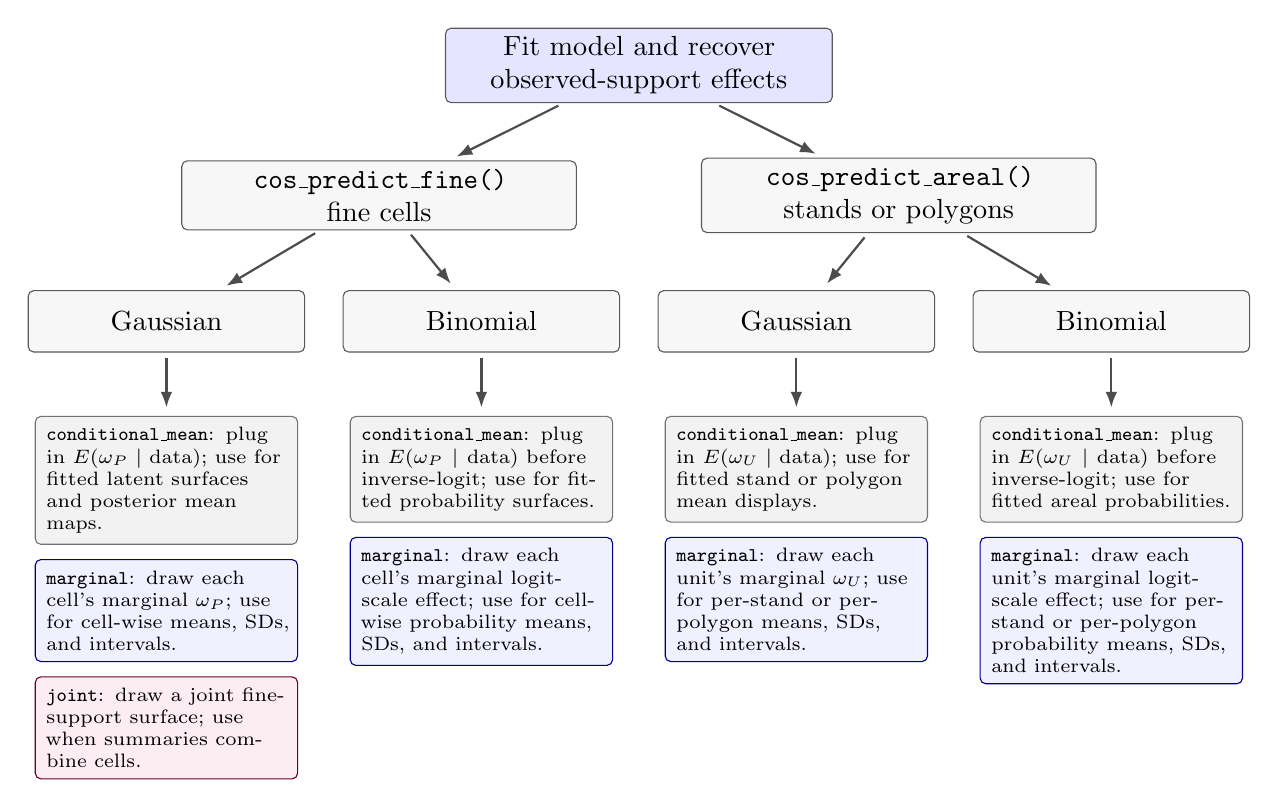
\begin{tikzpicture}[
  x=1cm,
  y=1cm,
  box/.style={
    rectangle,
    rounded corners=2pt,
    draw=black!65,
    fill=black!3,
    align=center,
    text width=3.3cm,
    minimum height=0.78cm,
    inner sep=3pt
  },
  decision/.style={
    diamond,
    aspect=1.75,
    draw=black!70,
    fill=blue!7,
    align=center,
    text width=2.6cm,
    inner sep=1pt
  },
  plug/.style={
    rectangle,
    rounded corners=2pt,
    draw=black!55,
    fill=black!5,
    align=left,
    text width=3.05cm,
    font=\scriptsize,
    anchor=north,
    inner sep=4pt
  },
  marg/.style={
    rectangle,
    rounded corners=2pt,
    draw=blue!55!black,
    fill=blue!6,
    align=left,
    text width=3.05cm,
    font=\scriptsize,
    anchor=north,
    inner sep=4pt
  },
  joint/.style={
    rectangle,
    rounded corners=2pt,
    draw=purple!55!black,
    fill=purple!7,
    align=left,
    text width=3.05cm,
    font=\scriptsize,
    anchor=north,
    inner sep=4pt
  },
  arrow/.style={-{Latex[length=2mm]}, thick, draw=black!70, shorten <=2pt, shorten >=3pt}
]
\node[box, fill=blue!10, text width=4.7cm] (start) at (0, 0)
  {Fit model and recover observed-support effects};

\node[box, text width=4.8cm] (fine) at (-3.3, -1.65)
  {\texttt{cos\_predict\_fine()}\\fine cells};
\node[box, text width=4.8cm] (areal) at (3.3, -1.65)
  {\texttt{cos\_predict\_areal()}\\stands or polygons};

\node[box] (fg) at (-6.0, -3.25)
  {Gaussian};
\node[box] (fb) at (-2.0, -3.25)
  {Binomial};
\node[box] (ag) at (2.0, -3.25)
  {Gaussian};
\node[box] (ab) at (6.0, -3.25)
  {Binomial};

\node[plug] (fgmean) at (-6.0, -4.45)
  {\texttt{conditional\_mean}: plug in \(E(\omega_P \mid \mathrm{data})\); use for fitted latent surfaces and posterior mean maps.};
\node[marg, below=0.18cm of fgmean] (fgmarg)
  {\texttt{marginal}: draw each cell's marginal \(\omega_P\); use for cell-wise means, SDs, and intervals.};
\node[joint, below=0.18cm of fgmarg] (fgjoint)
  {\texttt{joint}: draw a joint fine-support surface; use when summaries combine cells.};

\node[plug] (fbmean) at (-2.0, -4.45)
  {\texttt{conditional\_mean}: plug in \(E(\omega_P \mid \mathrm{data})\) before inverse-logit; use for fitted probability surfaces.};
\node[marg, below=0.18cm of fbmean] (fbmarg)
  {\texttt{marginal}: draw each cell's marginal logit-scale effect; use for cell-wise probability means, SDs, and intervals.};

\node[plug] (agmean) at (2.0, -4.45)
  {\texttt{conditional\_mean}: plug in \(E(\omega_U \mid \mathrm{data})\); use for fitted stand or polygon mean displays.};
\node[marg, below=0.18cm of agmean] (agmarg)
  {\texttt{marginal}: draw each unit's marginal \(\omega_U\); use for per-stand or per-polygon means, SDs, and intervals.};

\node[plug] (abmean) at (6.0, -4.45)
  {\texttt{conditional\_mean}: plug in \(E(\omega_U \mid \mathrm{data})\) before inverse-logit; use for fitted areal probabilities.};
\node[marg, below=0.18cm of abmean] (abmarg)
  {\texttt{marginal}: draw each unit's marginal logit-scale effect; use for per-stand or per-polygon probability means, SDs, and intervals.};

\draw[arrow] (start) -- (fine);
\draw[arrow] (start) -- (areal);
\draw[arrow] (fine) -- (fg);
\draw[arrow] (fine) -- (fb);
\draw[arrow] (areal) -- (ag);
\draw[arrow] (areal) -- (ab);
\draw[arrow] (fg) -- (fgmean);
\draw[arrow] (fb) -- (fbmean);
\draw[arrow] (ag) -- (agmean);
\draw[arrow] (ab) -- (abmean);
\end{tikzpicture}
}
\caption{Prediction uncertainty choices for Gaussian and binomial paths in
\texttt{cosTapered}. The key distinction is whether samples represent
conditional means, independent marginal uncertainty for each prediction unit,
or a joint fine-support Gaussian surface. Gray boxes are plug-in
conditional-mean summaries. Blue boxes are marginal prediction-unit summaries,
appropriate for stand, polygon, or cell estimates interpreted one unit at a
time. Purple boxes are joint fine-support samples for summaries that combine
cells. Runtime can differ substantially among paths, but the inferential
target should determine the choice.}
\label{fig:prediction_decision}
\end{figure}
\clearpage

\section{Missing raster cells and support targets}

Support weights define the estimand. If raster covariates are incomplete over
part of an observed or prediction polygon, dropping those cells changes the
support average. The default package behavior is therefore
\texttt{missing = "error"} when incomplete covariates would leave a support
row sum materially below one. Two explicit alternatives are available:
\begin{itemize}
\item \texttt{missing = "drop"} keeps the covered-cell weights without
  rescaling, so row sums may be below one.
\item \texttt{missing = "renormalize"} rescales the retained weights to sum to
  one, changing the target to the covered-cell average.
\end{itemize}
These choices should be made as modeling decisions, not as preprocessing
accidents.

\section{Path for future response models}

The support-weight machinery is largely independent of the response model.
Future response models should reuse the same objects \(\bH_{BA}\),
\(\bH_{UA}\), \(\bX_B\), and support-weight diagnostics where possible. The
parts likely to change are:
\begin{itemize}
\item the observation distribution for \(\by_B\);
\item the latent linear predictor or link function;
\item the sampler used for covariance and latent-effect updates;
\item the posterior predictive distribution for observed targets.
\end{itemize}
The distinction between latent support averages and observed support
responses should remain explicit for any new response family.

\bibliographystyle{plainnat}
\bibliography{cosTapered}

\end{document}
